\documentclass[3p,times,procedia,number]{elsarticle}
\flushbottom

%% The `ecrc' package must be called to make the CRC functionality available
\usepackage{ecrc}
%\usepackage{amsmath}
\volume{00}

%% set the starting page if not 1
\firstpage{1}

%% Give the name of the journal
\journalname{Procedia Engineering}

%% Give the author list to appear in the running head
\runauth{K. Kumar, J.-Y. Delenne and K. Soga}

%% Give the abbreviation of the Journal.
\jid{proeng}

%% End of ecrc-specific commands
%%%%%%%%%%%%%%%%%%%%%%%%%%%%%%%%%%%%%%%%%%%%%%%%%%%%%%%%%%%%%%%%%%%%%%%%%%
\usepackage{cleveref}
\graphicspath{figs/}
% ***************************** Math and SI Units ******************************
\usepackage{amsfonts}
\usepackage{amsmath}
\usepackage{amssymb}
\usepackage[per=slash]{siunitx} % use this package module for SI units
\usepackage{flexisym}
\usepackage{subcaption}

\biboptions{sort&compress}

% if you have landscape tables
\usepackage[figuresright]{rotating}

\begin{document}

\begin{frontmatter}


\dochead{1st International Conference on the Material Point Method, MPM 2017}

\title{Transient dynamics of granular slopes: MPM v DEM}

\author[a]{Krishna Kumar\corref{cor1}}
\author[a,b]{Kenichi Soga}
\author[c]{Jean-Yves Delenne}
\author[c,d]{Farhang Radjai}

\address[a]{Department of Engineering, University of Cambridge, Cambridge CB2
  1PZ, UK}
\address[b]{Department of Civil Engineering, University of California,
  Berkeley, USA}
\address[c]{University of Montpellier II, France}
\address[d]{Massachusetts Institute of Technology, Cambridge, USA}

\begin{abstract}
Transient granular flows, such as rock falls, debris flows, and aerial and
submarine avalanches, occur very often in nature. In the geotechnical
context, transient movements of large granular slopes are a substantial
factor of risk due to their destructive force and the transformations they
may produce in the landscape. This paper investigates the ability of MPM, a
continuum approach, to reproduce the evolution of a granular slope
destabilised by an external energy source. In particular, a central issue is
whether the power-law dependence of run-out distance and time observed with
respect to the initial geometry or energy can be reproduced by a simple
Mohr-Coulomb plastic behaviour. The effect of base 
friction on the run-out kinematics is studied by comparing the data obtained
from the DEM and MPM simulations. The mechanism of energy dissipation is
primarily through friction and the MPM is able to predict the run-out response in
good agreement with the DEM simulations. At very low excitation energies, 
the DEM simulations show longer run-out in comparison to the MPM due to local
destabilization at the flow front. At low input energies, a larger fraction of
the energy is consumed in the destabilisation process, hence the amount energy
available for flow is less. However, at higher input energy, where most of
the energy is dissipated during the spreading phase, the run-out distance 
has a weak dependence on the distribution of velocity in the granular mass.
\end{abstract}

\begin{keyword}
MPM; Granuar dynamics; Tranient flows; Continuum; 
Discrete Element Modelling;

%% PACS codes here, in the form: \PACS code \sep code

%% MSC codes here, in the form: \MSC code \sep code
%% or \MSC[2008] code \sep code (2000 is the default)

\end{keyword}
\cortext[cor1]{Corresponding author. Tel.: +44-1223 748589.}
\end{frontmatter}

\email{kks32@cam.ac.uk}

%% Start line numbering here if you want
% \linenumbers

%% main text

%\enlargethispage{-7mm}
\section{Introduction}
\label{sec:intro}
Transient granular flows occur very often in nature. Well-known examples are
rockfalls, debris flows, and aerial and submarine avalanches. They form a major
element of reshaping the lanscape and their high destructive potential is a
substantial factor of risk. Natural granular flows may be triggered as a result
of different processes such as gradual degradation, induced by weathering or
chemical reactions, liquefaction and external forces such as earthquakes.          

Granular flows have been studied in laboratory experiments in different 
geometries such as tilted slopes leading to slope failure and surface
avalanches~\citep{Mutabaruka2015,Legros2002, Iverson1997} or by considering
vertical columns of grains collapsing and spreading under their
ownweight~\citep{Lajeunesse2004, Lajeunesse2005}. The dynamics observed in
the experiments is often nontrivial in the sense that the final configurations
after the dissipation of the whole kinetic energy can not be readily predicted
by means of simple laws based on the Mohr-Coulomb nature of the material. For
example, in collapsing columns, the runout distance is found to obey a
power-law dependence with the initial aspect ratio of the column. 

The observed nontrivial transient dynamics is often correctly reproduced by the
discrete element method (DEM), which provides a powerful tool for the
grain-scale analysis of the trigger and its subsequent
dynamics~\citep{Staron2005, Staron2009}. However, even in simplified geometries
such as those investigated in the experiments, the DEM suffers from a
serious short-coming in the number of particles that can be simulated in a
reasonnable time. This is a critical issue when more complex geometries or
long-time granular processes are considered, or when particle size
distributions are broad. For this reason, most numerical studies are performed
in 2D or simple particles shapes and size distributions are considered. 

It is also obvious that classical modeling strategies based on the finite
element method (FEM) cannot be used for the simulation of very large
deformations. In various application of FEM, this problem is treated by means
of technical tools such as remeshing. Such methods are, however, not robust and
lead to round-off errors and mesh-senstitivity. In contrast, the 
Material Point Method (MPM) is an alternative approach for continuum problems
that allows for indefinitely large deformations without 
remeshing~\citep{Soga2016, Bandara2014, Bardenhagen2000, Sulsky1995}. In this
method, the material points carry the information on state variables and a
background fixed grid is used to solve the governing equations. The information 
between the material points and the grid is exchanged via suitable shape
functions. The MPM has been applied with success to a number of solid mechanics
problems and its theoretical foundations have recently been invesitgated by
several authors. 

In this paper, we investigate the ability of the MPM, as a continuum
approach, to reproduce the evolution of a granular slope
when destabilized by energy input. In particular, a central issue is wheather
power-law dependence of the runout distance and timewith respect to the initial
geometry or energy can be reproduced by a simple prescription of the
Mohr-Coulomb plastic behavior within a  MPM code. We therefore perform
extensive simulations by varying continuously different input parameters and
compare the data with those obtained from DEM simulations of the same system.
We compare in detail the evolution of the profile of the slope and its total
kinetic energy between the two methods and for differerent initial states. As
we shall see, the MPM can successfully simulate  the transient evolution with a
single input parameter, namely the internal angle of friction. This opens the
way to the simulation of geological-scale flows on complex topographies. 

\subsection{Numerical set-up}
\label{sec:num}

The DEM sample was composed of $\sim13000$ disks with a uniform distribution of 
diameters by volume fractions ($d_{max} = 1.5 d_{min}$). The mean grain 
diameter and mass are $d\simeq 2.455 $~\si{\mm} and $m\simeq 0.0123$~\si{\kg}, 
respectively. The grains are first poured uniformly into a rectangular box of 
given width and then the right-hand side wall is shifted far to the right 
to allow the grains to spread. A stable granular slope of 13.2~\si{\degree} is 
obtained when all grains come to rest. The initial slope configuration is shown
in~\cref{fig:slope_configuration}. This 
procedure leads to a mean packing fraction $\simeq 0.82$. Soil grains with a 
mean density of 2600~\si{\kg\per\m\cubed} and internal friction coefficient of 
0.4 between grains are considered. For grain-scale simulations, classical DEM
approach was used~\citep{Cundall1979a}. 

\begin{figure}[tbhp]
  \centering
  \begin{subfigure}[b]{0.47\textwidth}
    \centering
    \includegraphics[width=0.95\textwidth]{figs/slope_configuration}
    \caption{DEM}
    \label{fig:dem_slope_configuration}
  \end{subfigure}
  \begin{subfigure}[b]{0.47\textwidth}
    \centering
    \includegraphics[width=0.95\textwidth]{figs/mpm_velocity_slope}
    \caption{MPM}
    \label{fig:mpm_slope_setup}
  \end{subfigure}
  \caption{Initial geometry and dimensions of the slope subjected to a horizontal 
    velocity of 50J.}
  \label{fig:slope_configuration}
\end{figure}


In the present study, Generalised Interpolation Material Point Method 
is used to avoid cell crossing noise~\citep{Steffen2008, Bardenhagen2004}.
In MPM simulations, the material point spacing is adopted to be the same as the 
mean grain diameter in DEM. A mesh size of 0.0125m is adopted with 25 material 
points per cell. The effect of mesh size and the number of material points per 
cell was investigated by~\citet{Soundararajan2015}. The initial configuration
of the slope used in the MPM simulations is shown in~\cref{fig:mpm_slope_setup}.
Frictional boundary conditions are applied on the left and the bottom boundaries
by applying constraints to the nodal acceleration. Mohr-Coulomb model with no
dilation is used to simulate the continuum behaviour of the granular slope.
Periodic shear tests in DEM reveals a macroscopic friction coefficient of 0.22.
Further details about DEM and MPM parameters and set-up can be found in
~\citet{Soundararajan2015}.

The initial static slope was set into motion by applying a horizontal
gradient velocity $v_{0x}(y) = k (y_{max} - y)$ with $k>0$. The evolution of 
the slope geometry and the total kinetic energy as a function of the initial 
input energy $E_0$ is studied. The run-out distance $L_f$ is the distance of 
the rightmost grain, which is still in contact with the main mass when the slope 
comes to rest. The run-out will be normalised by the initial length $L_0$ of 
the slope, as in the experiments of collapsing columns. The total run-out 
duration $t_f$ is the time taken by the slope to reach its final run-out 
distance $L_f$.

The natural units of the system are the mean grain diameter $d$, the mean grain 
mass $m$ and acceleration due to gravity $g$. For this reason, the length 
scales are normalised by $d$, time by $(d/g)^{1/2}$, velocities by $(gd)^{1/2}$ 
and energies by $mgd$. 

%-------------------------------------------------------------------------------
\subsection{Evolution of slope geometry and run-out}
\label{sec:evolution}

\Cref{fig:mpm_gradvelocity_200j} shows the initial evolution of the 
granular slope subjected to an initial horizontal energy $E_0 = 61$ (in 
dimensionless units) using MPM. As the granular slope is sheared along the 
bottom, the shear propagates to the top leaving a cavity in the vicinity of the 
left wall. This cavity gets partially filled as the granular mass at the top 
collapse behind the flowing mass due to inertia. Similar behaviour is observed 
during the initial stages of the flow evolution using DEM  
(\cref{fig:dem_gradvelocity_200j}). Due to inertia, the grains at the top 
of the granular heap roll down to fill the cavity, while the slope continues to 
spread. 

\begin{figure}[tbph]
  \centering
  \begin{subfigure}[b]{0.47\textwidth}
    \centering
    \includegraphics[width=\textwidth]{figs/mpm_gradvelocity_200j}
    \caption{MPM}
    \label{fig:mpm_gradvelocity_200j}
  \end{subfigure}
  \begin{subfigure}[b]{0.42\textwidth}
    \centering
    \includegraphics[width=\textwidth]{figs/dem_gradvelocity_200j}
    \caption{DEM}
    \label{fig:dem_gradvelocity_200j}
  \end{subfigure}
  \caption{Evolution of granular slopes subjected to a gradient
    horizontal energy $E_0/(mgd)$ of 61.}
  \label{fig:gradvelocity_200j}
\end{figure}


The flow involves a transient phase with a change in the geometry of the slope 
followed by continuous spreading. The gradient of input energy applied to the 
granular slope mimics a horizontal quake. Despite the creation of a cavity
behind the flowing mass, the granular heap remains in contact with the left
wall irrespective of the input energy.~\Cref{fig:runout_eo_mpm_dem} shows the
normalised run-out distance $(L_f - L_0)/L_0$ and total run-out time $t_f$ as a
function of the input energy $E_0$. Two regimes characterised by a power-law
relation between the run-out distance and time as a function of $E_0$ can be
observed. In the first regime, corresponding to the range of low input energies
$E_0 < 40 \ mgd$, the run-out distance observed varies as $L_f \propto
(E_0)^\alpha$ with $\alpha \simeq 0.206 \pm 0.012$ over nearly one log cycle.
Overall, the run-out distance predicted by the continuum approach matches the
DEM simulations. At very low energies, DEM simulations show longer run-out
distance due to local fluidisation.


While the run-out exhibits a power-law relation with the initial input energy, 
the DEM simulations show that the flow duration remains constant at a value  
$t_f \simeq 60 \  (d/g)^{0.5}$ irrespective of the value of $E_0$. The constant 
run-out time, in grain-scale simulations, indicates the collapse of grain into 
the cavity left behind the slope. An average run-out speed can be defined as 
$v_s = (L_f - L_0) / t_f$. According to the data, $v_s \propto 
(E_0)^{0.52\pm 0.012}$. The error on the exponent represents the error due to
the linear fit on the logarithmic scale. Since the initial average velocity
varies as $v_0 \propto (E_0)^{0.5}$, this difference between the values of the
exponents suggests that the mobilised mass during run-out declines when the
input energy is increased.


\begin{figure}[tbph]
  \centering
  \begin{subfigure}[b]{0.49\textwidth}
    \centering
    \includegraphics[width=\textwidth]{figs/runout_eo_mpm_dem}
    \caption{Run-out as a function of $KE_0$.}
    \label{fig:runout_eo_mpm_dem}
  \end{subfigure}
  \begin{subfigure}[b]{0.49\textwidth}
    \centering
    \includegraphics[width=\textwidth]{figs/Tf_vs_Eo_Slope}
    \caption{Duration of run-out as a function of $KE_0$.}
    \label{fig:Tf_vs_Eo_Slope}
  \end{subfigure}
  \caption{Evolution of run-out and time as a function of the normalised input 
  energy for a slope subjected a gradient horizontal energy.}
  \label{fig:Slope}
\end{figure}

In the second regime, corresponding to the range of high input energies  $E_0 > 
40 \ mgd$, the run-out distance varies as $L_f \propto (E_0)^{\alpha'}$ over 
one cycle with $\alpha' \simeq 0.56\pm 0.04$ while the duration increases as 
$t_f \propto (E_0)^{\beta'}$ with $\beta' \simeq 0.33 \pm 0.02$. Hence, in this 
regime the average run-out speed varies as $v_s \propto (E_0)^{0.498 \pm 
0.01}$. This exponent is close to the value $0.5$ in $v_0 \propto (E_0)^{0.5}$, 
and hence, within the confidence interval of the exponents.
In the second regime, both DEM and MPM predict almost the same run-out 
behaviour. However, the MPM predicts longer duration with increase in the input 
energy.

It is worth noting that a similar power-law dependence of the run-out distance 
and time are found in the case of granular column collapse with respect to 
the initial aspect ratio. In the column geometry, the grains spread away 
owing to the kinetic energy acquired during gravitational collapse of the 
column.~\citet{Topin2012} found that the run-out distance varies as a power-law 
of the available peak kinetic energy at the end of the free-fall stage with an 
exponent $\simeq 0.5$. This value of exponent is lower than the run-out 
evolution observed in the second regime. This is, however, physically plausible 
since the distribution of kinetic energies at the end of the collapse 
is more chaotic than in this case where the energy is supplied from the very 
beginning in a well-defined shear mode. As pointed out by~\citet{Staron2005}, 
the distribution of kinetic energies is an essential factor for the run-out 
distance.

%-------------------------------------------------------------------------------------------
\subsection{Decay of kinetic energy}
\label{sec:decay}

The non-trivial evolution of the slope geometry in two regimes suggests that 
the energy supplied to the slope is not simply dissipated by shear and friction 
along the bottom plane. It is important to split the kinetic energy into 
vertical and horizontal components ($K_{Ex}$ and $K_{Ey}$) of the velocity 
field. Although, the input energy is in the $x$ component, a fraction of 
the energy is transferred to the vertical component of the velocity field and 
dissipated during the transient phase. The evolution of kinetic energy is 
studied to understand the behaviour of granular flow that is consistent with 
the evolution of the slope shape.

The evolution of total kinetic energies $E_k$ with time for different values of 
the input energy $E_{ki}$ based on MPM simulations are shown 
in~\cref{fig:Energy_Time_Slope}. The MPM simulation shows two distinct regimes 
in the normalised kinetic energy plot as a function of normalised time 
in~\cref{fig:Normalised_Energy_Time_Slope_MPM}. However, the DEM simulations 
(\cref{fig:Normalised_Energy_Time_Slope_DEM}) show that the energy evolution 
corresponding to the low energy regime nearly collapse on to a single time 
evolution. This is consistent with the observation of run-out time $t_f$ being 
almost independent of the input energy. In contrast, MPM simulations predict a power 
law relation between the run-out duration and input energy. However, the 
plots corresponding to the high energy regime (\cref{fig:Energy_Time_Slope}), 
collapse only at the beginning of the run-out i.e. for $t < t_1 \simeq 7.5 \ 
(d/g)^{0.5}$. Although MPM simulations show a longer duration of run-out 
(\cref{fig:Energy_Time_Slope}), the total kinetic energy is completely 
dissipated at $t = 60 \sqrt{d/g}$. DEM simulations predict $t = 80 \sqrt{d/g}$ 
for the kinetic energy to be completely dissipated, which is due to grain 
rearrangement at the free surface. The granular mass densifies as the flow
progresses, after the initial dilation phase for $t = 20\sqrt{d/g}$.

\begin{figure}[tbhp]
  \centering
  \begin{subfigure}[b]{0.4\textwidth}
    \centering
    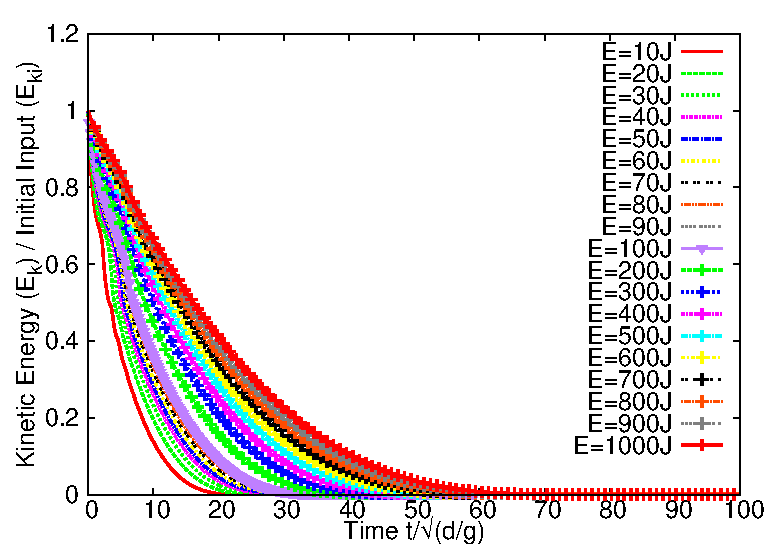
\includegraphics[width=\textwidth]{figs/Normalised_Energy_Time_Slope_MPM}
    \caption{MPM}
    \label{fig:Normalised_Energy_Time_Slope_MPM}
  \end{subfigure}
  \begin{subfigure}[b]{0.4\textwidth}
    \centering
    \includegraphics[width=\textwidth]{figs/Normalised_Energy_Time_Slope_DEM}
    \caption{DEM}
    \label{fig:Normalised_Energy_Time_Slope_DEM}
  \end{subfigure}
  \caption{Evolution of normalised kinetic energy with normalised time for a
  slope subjected to gradient input velocities.}
  \label{fig:Energy_Time_Slope}
\end{figure}

\Cref{fig:Normalised_KEx_KEy_Slope} displays the evolution of kinetic energy 
in the translational ($E_x$ and $E_y$) degrees of freedom. $E_x$ decays similar 
to the total energy dissipation, but $E_y$ increases and passes through a peak 
before decaying rapidly to a negligible level. The transient is best 
observed for $E_y$, which has significant values only for $t< t_1$. This energy 
represents the proportion of kinetic energy transferred to the $y$ component of 
the velocity field  due to the destabilisation of the slope and collapse of 
grains in the cavity behind the slope. Higher proportion of vertical 
acceleration $E_{ky}/E_0$ is observed for lower values of input energy $E_0$. 
This means that, at lower input energies a larger fraction of the energy is 
consumed in the destabilisation process. Whereas at a higher input energies, 
most of the energy is dissipated in the spreading phase. For this reason, the 
total duration $t_1$ of this destabilisation phase is nearly the same in 
both regimes and its value is controlled by gravity rather than the input 
energy. The height of the slope being of the order of $80 \ d$, the total 
free-fall time for a particle located at this height is $\simeq 12 \ 
(d/g)^{0.5}$, which is of the same order as $t_1$. DEM simulations show that 
the contribution of the rotational energy during the transient stage and the 
spreading stage is negligible. 

\begin{figure}[tbhp]
  \centering
  \begin{subfigure}[b]{0.4\textwidth}
    \includegraphics[width=\textwidth]{figs/Normalised_KEx_Slope}
    \caption{Evolution of normalised horizontal kinetic energy with time.}
    \label{fig:Normalised_KEx_Slope}
  \end{subfigure}
  \begin{subfigure}[b]{0.4\textwidth}
    \centering
    \includegraphics[width=\textwidth]{figs/Normalised_KEy_Slope}
    \caption{Evolution of normalised vertical kinetic energy with time.}
    \label{fig:Normalised_KEy_Slope}
  \end{subfigure}
  \caption{Evolution of vertical and horizontal kinetic energy with time (MPM) 
  for a slope subjected to gradient input velocities.}
  \label{fig:Normalised_KEx_KEy_Slope}
\end{figure}

To analyse the second phase for higher input energies, the kinetic energy
$E'_{kx0}$ at the end of the transient phase is considered. This energy is
responsible for most of the run-out, hence it is expected to control the
run-out distance and time. A decay time $\tau$ can be defined as the time
required for $E_{kx}$ to decline by afactor $1/2$.~\Cref{fig:ExEx0_vs_ttau}
shows the same data in which the time $t'$ elapsed since $t_1$, normalised by
$\tau$. Interestingly, now all the data nicely collapse on to a single curve.
However, this curve can not be fitted by simple functional forms such as
variants of exponential decay. This means that the spreading of the slope is not
a self-similar process in agreement with the fact that the energy fades away in
a finite time $t'_f$. 

\begin{figure}[tbhp]
  \centering
  \includegraphics[width=0.4\textwidth]{figs/EkxKoTTau_Slope}
  \caption[Evolution of the normalised horizontal kinetic energy as function of 
  the normalised time since the transient phase.]{Evolution of kinetic energy in 
  the $x$ component of the velocity field  normalised by the available kinetic
  energy at the end of the transient as a function of normalised time (MPM).}
  \label{fig:ExEx0_vs_ttau}
\end{figure}


The scaling of the data with the decay time $\tau$ suggests that the 
run-out time, since the beginning of the second phase, $t'_f$ might be a simple 
function of $\tau$.~\Cref{fig:tp_tau_mgd} shows both $t'_f$ and $\tau$ as 
a function of $E'_{x0}$, where a power-law relation can be observed for both 
time scales. The run-out time $t'_f \propto (E'_{x0})^{\beta'}$ has the 
same exponent $\beta' \simeq 0.33 \pm 0.02$ as $t_f$ as a function of $E_0$. 
For the decay time we have $\tau \propto (E'_{x0})^{\beta''}$ with $\beta'' 
\simeq 0.38 \pm 0.03$. The relation between the two times can thus be expressed 
as (\cref{fig:tp_tau})
\begin{equation}
  t'_f = k  \ \tau \, (E'_{x0})^{\beta'' - \beta'} \,,
  \label{eqn:t'f}
\end{equation}
where $k \simeq 5.0 \pm 0.4$ and $\beta'' - \beta' \simeq 0.05 \pm 0.05$. This 
value is small enough to be neglected. It is therefore plausible to assume that 
the run-out time is a multiple of the decay time and the spreading process is 
controlled by a single time. A weak dependence on the energy $E'_{kx0}$ is 
consistent with the fact that the energy available at the beginning of the 
second phase is not dissipated in the spreading process (calculated from the 
position of the tip of the slope) since the slope keeps deforming by the 
movements of the grains at the free surface even when the tip comes to rest. 
This can explain the small difference between the two exponents as observed 
here.

\begin{figure}[tbhp]
  \centering
  \begin{subfigure}[b]{0.4\textwidth}
    \includegraphics[width=\textwidth]{figs/tp_tau_mgd}
    \caption{}
    \label{fig:tp_tau_mgd}
  \end{subfigure}
  \begin{subfigure}[b]{0.4\textwidth}
    \centering
    \includegraphics[width=\textwidth]{figs/tp_tau}
    \caption{}
    \label{fig:tp_tau}
  \end{subfigure}
  \caption{Decay time and run-out time as a function of the normalised kinetic 
  energy $E_{kx0}$: (a) Power law evolution of $t'_f$ and $\tau$ as a function
  of kinetic energy $E'_{kx0}$ and (b) Linear relationship between decay time
  and run-out time after the transient as a function of the normalised kinetic
  energy $E_{kx0}$.}
  \label{fig:tp_Tau}
\end{figure}


%-------------------------------------------------------------------------------
\subsection{Effect of friction}
\label{sec:parameters}

The run-out distance, duration of flow, and the dissipation of kinetic energy 
are controlled by the input energy and collective dynamics of the whole slope. 
However, the run-out behaviour is also expected to depend on the base friction. 
A series of simulations with different values of base friction was performed 
using MPM to analyse the influence of friction on the run-out behaviour. The 
influence of friction on the run-out behaviour for different input energies is 
shown in~\cref{fig:runout_fric_slope}. The run-out distance decreases with 
increase in the basal friction. The exponent of the 
power-law relation between the run-out and input energy has a weak dependence 
on the base friction, however, the proportionality constant is affected by the 
change in the base friction. This behaviour is similar to that observed in 
granular column collapse with varying initial 
properties~\citep{Balmforth2005,Lajeunesse2005}. 

The effect of friction coefficient is quite important for the run-out. MPM
simulations with varying friction coefficient show that both the run-out
distance and the decay time decrease as the friction coefficient is increased.
This effect is much more pronounced at low values of the friction coefficient.
The run-out time, for example, is reduced by a factor of approximately 4 as
$\mu_s$ is increased from 0.1 to 0.2 while the change in the run-out and
duration is less affected with increase in friction coefficient. This
``saturation effect'' can be observed in a systematic way in simple shear
tests. The dissipation rate may reach a saturation point where the dilation of
granular materials and rolling of the grains change in response to increase in
friction coefficient~\citep{Estrada2008}.

\begin{figure}[tbhp]
  \centering
  \begin{subfigure}[b]{0.4\textwidth}
    \centering
    \includegraphics[width=\textwidth]{figs/runout_fric_slope}
    \caption{run-out distance}
    \label{fig:runout_fric_slope}
  \end{subfigure}
  \begin{subfigure}[b]{0.4\textwidth}
    \centering
    \includegraphics[width=\textwidth]{figs/time_fric_slope}
    \caption{duration of run-out}
    \label{fig:time_fric_slope}
  \end{subfigure}
  \caption{MPM simulations of effect of friction on the run-out behaviour of 
  slopes subjected to horizontal excitation.}
  \label{fig:fric_slope}
\end{figure}

\section{Conclusion}
Natural granular flows are triggered by different mechanisms. The distribution 
of kinetic energy in the granular mass is found to have an effect on the flow 
kinematics. A multi-scale analyses of a granular slope subjected to horizontal 
velocities are performed and the following conclusions are derived:

\begin{itemize}

  \item A power-law dependence of the run-out distance and time as a 
    function of the input energy is observed. The power-law behaviour is found to 
    be a generic feature of granular flow dynamics. The values of the power-law
    exponents are not simple functions of the geometry. 

  \item Two regimes with different values of the exponents: 
    a low-energy regime and a high-energy regime are observed. 

  \item The low energy regime reflects mainly the destabilisation of the slope, 
    with a run-out time independent of the input energy.

  \item The second regime is governed by the spreading dynamics 
    induced by higher input energy. The evolution of granular slope in the 
    high-energy regime can be described by a characteristic decay time, which is 
    the time required for the input energy to decay by a factor of 0.5.

  \item The run-out distance and the decay time decrease as the friction 
    increases. This effect is much more pronounced at low values of friction.

  \item  At low input energies, the distribution of kinetic energy in the system is 
    found have a significant effect on the run-out, as the energy is mostly 
    consumed in the destabilisation process. 
     
  \item At higher input energies, where most of the energy is dissipated during 
    the spreading phase, the run-out distance has a weak dependence on the 
    distribution of velocity in the granular mass. 

  \item The material property and the distribution of kinetic energy in the 
    system has a non-trivial influence on the flow kinematics and the internal flow 
    structure.

  \item MPM is successfully able to simulate the transient evolution with a 
    single input parameter, the macroscopic friction angle.

\end{itemize}

This study exemplifies the ability of MPM, a continuum approach,  in modelling 
complex granular flow dynamics and opens the possibility of realistic 
simulation of geological-scale flows on complex topographies.

\section*{Acknowledgements}
The authors would like to thank Professor F. Radjai, LMGC, Montpellier, France for stimulating discussions regarding this work. The author would like to thank the Cambridge Commonwealth and Overseas Trust for the financial support to the first author to pursue this research. 

\bibliographystyle{model1-num-names}
\bibliography{references} 
\end{document}

%% End of file `procs-template.tex'.
